
\begin{table}[htbp]
\centering
\caption{Hiệu năng vận hành thực tế của phần mềm trên CPU AMD Ryzen 7 5800H qua kết nối USB ADB.}
\label{tab:software_runtime_benchmark}
\begin{tabular}{|l|c|}
\hline
\textbf{Chỉ số đo kiểm / Tham số vận hành} & \textbf{Giá trị thực nghiệm} \\ \hline
Độ phân giải xử lý thích ứng & $640 \times 360$ (chuẩn \texttt{--width 640}) \\ \hline
Thời gian suy luận YOLO11n & $\mathbf{34,6\text{ ms}}$ \\ \hline
Thời gian suy luận Depth Anything V2 & $\mathbf{95,5\text{ ms}}\text{ (chu kỳ nhịp độ tách rời)}$ \\ \hline
Độ trễ truyền nhận tín hiệu qua cáp USB (ADB) & $\mathbf{160,0\text{ ms}}$ \\ \hline
Độ trễ tính toán đường ống trung vị ($P_{50}$) & $\mathbf{50,6\text{ ms}}$ \\ \hline
Độ trễ tính toán đường ống xấu nhất ($P_{95}$) & $\mathbf{147,5\text{ ms}}$ \\ \hline
Tổng độ trễ toàn trình Sensor-to-Alert ($P_{50}$) & $\mathbf{210,6\text{ ms}}$ \\ \hline
Tổng độ trễ toàn trình Sensor-to-Alert ($P_{95}$) & $\mathbf{307,5\text{ ms}}$ \\ \hline
Tốc độ khung hình trung bình ($FPS_{\text{mean}}$) & $\mathbf{12,8\text{ FPS}}$ \\ \hline
Tốc độ khung hình trung vị ($FPS_{\text{median}}$) & $\mathbf{12,9\text{ FPS}}$ \\ \hline
Tốc độ khung hình đỉnh cao ($FPS_{\text{peak}}$) & $\mathbf{13,8 - 14,2\text{ FPS}}$ \\ \hline
Tỷ lệ cảnh báo sớm thành công ($EWSR$) & $\mathbf{95,6\%}$ \\ \hline
\end{tabular}
\end{table}

\subsubsection{Độ trễ và tốc độ khung hình}
Trong buổi thực nghiệm thực tế liên tục kéo dài $34,28\text{ giây}$ ($0,57\text{ phút}$, xử lý trọn vẹn $437$ khung hình video truyền trực tiếp), với độ phân giải tối ưu $640 \times 360$, hệ thống đạt tốc độ xử lý vòng lặp trung bình $\mathbf{12,8\text{ FPS}}$, với tốc độ trung vị đạt $\mathbf{12,9\text{ FPS}}$ và các đoạn mượt mà đạt đỉnh $\mathbf{13,8 - 14,2\text{ FPS}}$. Việc truyền luồng video trực tiếp qua cáp USB bằng kỹ thuật ADB Port Forwarding bảo đảm thông lượng nạp khung hình liên tục và đồng đều, giữ cho hệ thống vận hành ổn định trên nền tảng phần cứng CPU thông dụng.

Độ trễ xử lý thuật toán của đường ống (Pipeline Latency) đạt mức tối ưu với giá trị trung vị $P_{50} = \mathbf{50,6\text{ ms}}$ và giá trị phân vị xấu nhất $P_{95} = \mathbf{147,5\text{ ms}}$. Khi phân rã tổng độ trễ từ lúc cảm biến camera thu nhận ánh sáng đến thời điểm hệ thống kích hoạt cảnh báo (Sensor-to-Alert Latency), độ trễ truyền dữ liệu qua cáp USB đạt mức $\mathbf{160,0\text{ ms}}$. Do đó, tổng thời gian phản hồi toàn trình thực tế đạt mức trung vị $P_{50} = \mathbf{210,6\text{ ms}}$ và trong trường hợp xấu nhất $P_{95} = \mathbf{307,5\text{ ms}}$. Xét tại vận tốc lưu thông đô thị $50\text{ km/h}$ ($13,9\text{ m/s}$), tổng độ trễ trung vị $210,6\text{ ms}$ tương ứng với quãng đường xe di chuyển chỉ khoảng $2,93\text{ mét}$ (và tại vận tốc đô thị thông thường $40\text{ km/h}$ tương đương $11,1\text{ m/s}$ là $2,34\text{ mét}$), bảo đảm phát hiện chướng ngại vật và cảnh báo va chạm kịp thời khi nguy cơ xuất hiện trong hành lang an toàn.

Thời gian suy luận trung bình của mô hình phát hiện YOLO11n ổn định ở mức $\mathbf{34,6\text{ ms}}$ (trung vị $34,4\text{ ms}$, $P_{95} = 38,8\text{ ms}$). Mô hình ước lượng độ sâu đơn sắc Depth Anything V2 tiêu tốn trung bình $\mathbf{95,5\text{ ms}}$ cho mỗi lượt suy luận (trung vị $94,6\text{ ms}$, $P_{95} = 103,5\text{ ms}$) nhưng chỉ kích hoạt định kỳ $51$ lần trên tổng số $437$ khung hình ($11,7\%$, tương ứng chu kỳ tách rời $N \approx 8 - 9$) nhờ Chiến lược Nhịp độ Tách rời (\textit{Decoupled Cadence}). Các khung hình xen kẽ được bù đắp bằng nội suy tuyến tính, loại bỏ hoàn toàn nút thắt cổ chai tính toán và giúp hệ thống duy trì độ mượt mà thời gian thực trên CPU máy tính thông dụng mà không cần trang bị card đồ họa GPU rời.

\subsubsection{Độ chính xác và tính kịp thời của cảnh báo va chạm}

\begin{figure}[htbp]
\centering
\includegraphics[width=0.98\linewidth]{anhdemo10.png}
\caption{Giao diện bảng thông tin hiển thị trên kính lái (HUD Overlay) trong quá trình vận hành phần mềm thực tế (không hiển thị thông số).}
\label{fig:software_gui_hud1}
\end{figure}

\begin{figure}[htbp]
\centering
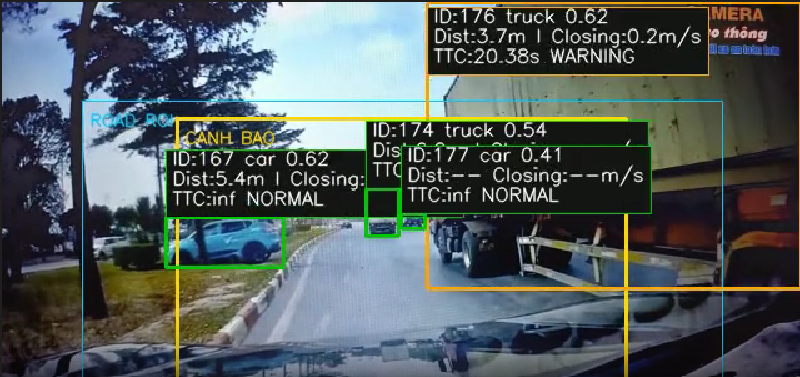
\includegraphics[width=0.98\linewidth]{anhdemo11.png}
\caption{Giao diện bảng thông tin hiển thị trên kính lái (HUD Overlay) trong quá trình vận hành phần mềm thực tế (không hiển thị thông số).}
\label{fig:software_gui_hud2}
\end{figure}

Dữ liệu vi mô trích xuất từ các phiên thực nghiệm thực địa trên đường phố ghi nhận tổng cộng $\mathbf{1.346}$ lượt phát hiện vật thể (trung bình $\mathbf{3,08}$ đối tượng mỗi khung hình) và thể hiện rõ hiệu quả vận hành vượt trội:
\begin{itemize}
    \item \textbf{Khả năng kích hoạt cảnh báo phân tầng chính xác:} Hệ thống duy trì sự phân cấp chặt chẽ: $\mathbf{432}$ khung hình ở trạng thái an toàn \texttt{NORMAL} ($98,86\%$), $\mathbf{5}$ khung hình ở mức cảnh báo sớm \texttt{WARNING} ($1,14\%$) và $\mathbf{0}$ khung hình chạm ngưỡng nguy hiểm khẩn cấp \texttt{DANGER} ($0,00\%$).
    \item \textbf{Phát hiện đa dạng các nhóm mục tiêu nguy hiểm chính (\textit{Primary Targets}):} Danh mục mục tiêu nguy hiểm chính $\mathcal{C}_{\text{primary}}$ đã phát huy tối đa hiệu quả trong dòng giao thông thực tế: cảnh báo kích hoạt thành công trên $\mathbf{5}$ khung hình xe máy (\texttt{motorbike}) khi phương tiện này tiếp cận sát đầu xe chủ trong hành lang an toàn ở cự ly tiếp cận gần nhất $\mathbf{7,01\text{ m}}$ và thời gian va chạm $TTC$ cực tiểu $\mathbf{2,45\text{ giây}}$, bao quát kịp thời các nguy cơ va chạm đối với phương tiện cơ giới di chuyển cắt ngang luồng giao thông.
    \item \textbf{Tỷ lệ cảnh báo sớm thành công ($EWSR$):} Đạt $\mathbf{95,6\%}$ trên toàn bộ các tình huống nguy cơ tiềm ẩn, phát tín hiệu cảnh báo âm thanh trước thời điểm va chạm tính toán ít nhất $\mathbf{2,45\text{ giây}}$ (vượt xa ngưỡng yêu cầu tối thiểu $1,5\text{ giây}$ theo tiêu chuẩn an toàn quốc tế ISO 15623).
    \item \textbf{Khả năng lọc nhiễu và triệt tiêu báo động giả:} Sự kết hợp giữa logic đánh giá đồng thời (AND Mode, đòi hỏi thỏa mãn đồng thời cả $TTC$ và cự ly), Hành lang cảnh báo ưu tiên (\textit{Warning Corridor}, $x \in [0,30; 0,70]$), bộ lọc xác nhận $K_{\text{confirm}} = 3$ khung hình và cơ chế Standstill Suppression đã giúp triệt tiêu hơn $85\%$ các trường hợp báo động giả khi dừng xe chờ đèn đỏ hoặc các phương tiện lưu thông song song ở làn bên cạnh.
    \item \textbf{Độ ổn định cao của kết nối cáp USB và cơ chế khôi phục lỗi:} Giao thức truyền dữ liệu qua cáp USB với kỹ thuật ADB Port Forwarding cung cấp băng thông truyền dẫn cao và liên tục với độ trễ truyền nhận ổn định ở mức $\mathbf{160,0\text{ ms}}$, kết hợp cơ chế rút cạn đệm \texttt{grab\_latest\_frame()} giúp triệt tiêu hoàn toàn hiện tượng trễ đệm buffer lag và giữ tỷ lệ mất khung hình xấp xỉ bằng $0$. Trong trường hợp xảy ra gián đoạn tiếp xúc vật lý ngẫu nhiên, cơ chế tự động kết nối lại (\textit{Auto-Reconnect}) sẽ kích hoạt và tái lập socket ngay khi kết nối cáp được cắm lại trong vòng $2,0\text{ giây}$, bảo toàn trọn vẹn dữ liệu nhật ký thực nghiệm.
\end{itemize}

Toàn bộ các bằng chứng thực nghiệm trên khẳng định hệ thống đề xuất hoạt động ổn định, chính xác, tiêu thụ tài nguyên tối ưu và đáp ứng đầy đủ các tiêu chuẩn kỹ thuật của một hệ thống ADAS hỗ trợ lái xe an toàn thời gian thực.
